\documentclass[12pt,a4paper]{article}
\usepackage[utf8]{vietnam}
\usepackage[top=2cm, bottom=1.5cm, left=2cm, right=1.45cm] {geometry}
\usepackage{amsmath,amsfonts,amssymb}
\usepackage{indentfirst,enumitem}
\usepackage{graphicx}
\usepackage{multicol}
\usepackage{setspace}
\usepackage{subfigure}


%CHÈN ẢNH
\usepackage{pgfplots}
\pgfplotsset{compat=1.15}
\usepackage{mathrsfs}
\usetikzlibrary{arrows}
\usetikzlibrary[patterns]

%----LẬT NGƯỢC CHỮ
\usepackage{rotating}
\newtheorem{answer}{Answer}
\usepackage{environ}
\NewEnviron{Answer}
{%
\noindent
\rotatebox[origin=c]{180}{%
\noindent
\begin{minipage}[t]{\linewidth}
\begin{answer}
\BODY
\end{answer}%
\end{minipage}%
}%
}%
%----LẬT NGƯỢC CHỮ
\usepackage{tikz,tkz-tab}
\begin{document}

\begin{titlepage}
    \begin{center}
        \vspace{7pt}
        \LARGE{CHUYÊN ĐỀ TOÁN MÁY TÍNH CẦM TAY CẤP THPT}
    \end{center}

    \vspace{30pt}
    %Here begins the 2D plot
    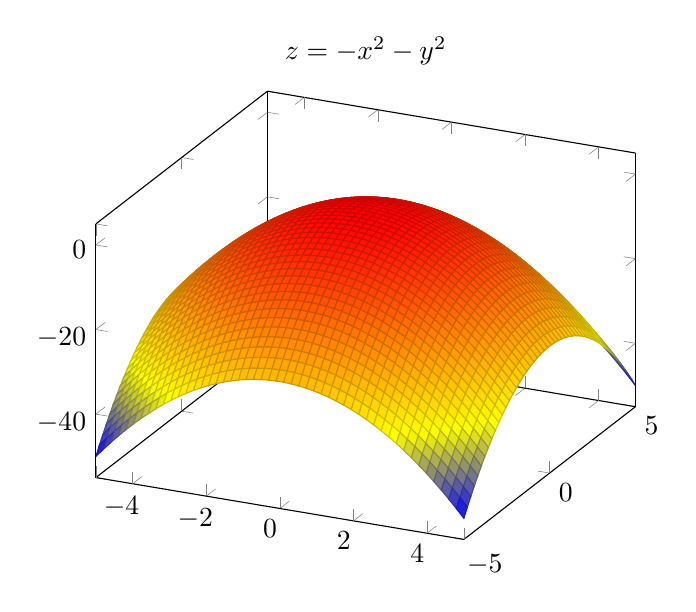
\begin{tikzpicture}
        \begin{axis}[title= \text{$z = -x^2-y^2$}]
        \addplot3[surf, samples = 50]{-x^2-y^2};
        \end{axis}
        \end{tikzpicture}
    %Here ends the 2D plot
    \hskip 10pt
    %Here begins the 3D plot
    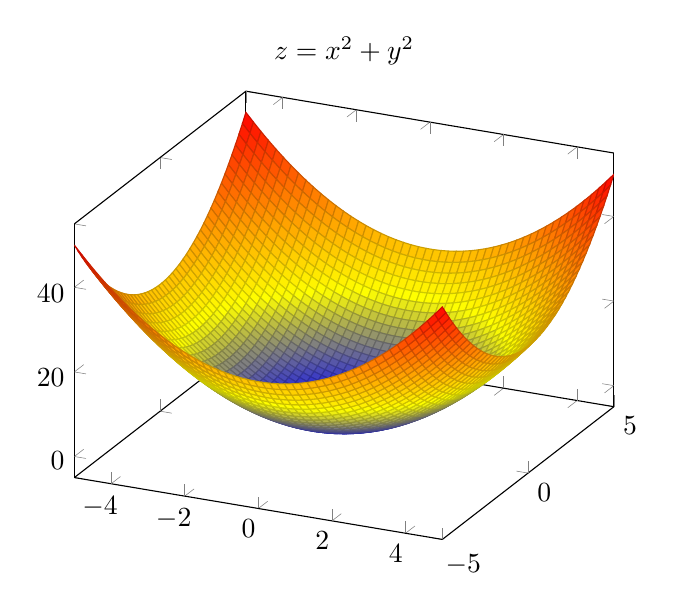
\begin{tikzpicture}
        \begin{axis}[title= \text{$z = x^2+y^2$}]
        \addplot3[surf, samples = 50]{x^2+y^2};
        \end{axis}
        \end{tikzpicture}
    \vspace{10pt}
    %Here begins the 2D plot
    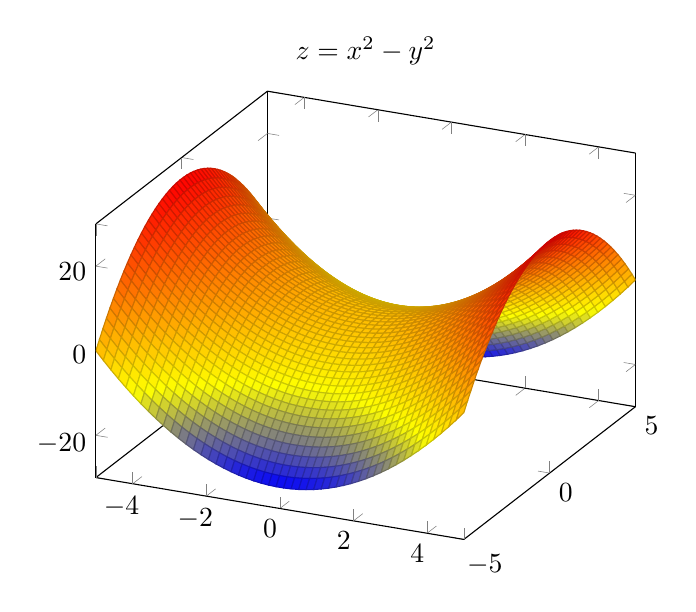
\begin{tikzpicture}
        \begin{axis}[title= \text{$z = x^2-y^2$}]
        \addplot3[surf, samples = 50]{x^2-y^2};
        \end{axis}
        \end{tikzpicture}
    %Here ends the 2D plot
    \hskip 10pt
    %Here begins the 3D plot
    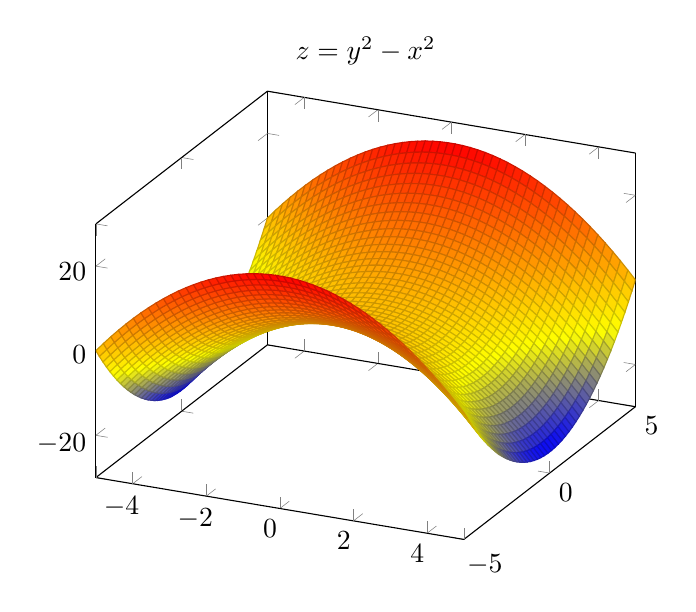
\begin{tikzpicture}
        \begin{axis}[title= \text{$z = y^2-x^2$}]
        \addplot3[surf, samples = 50]{y^2-x^2};
        \end{axis}
        \end{tikzpicture}
    \\
    \vspace{10pt}
    %Here begins the 3D plot
    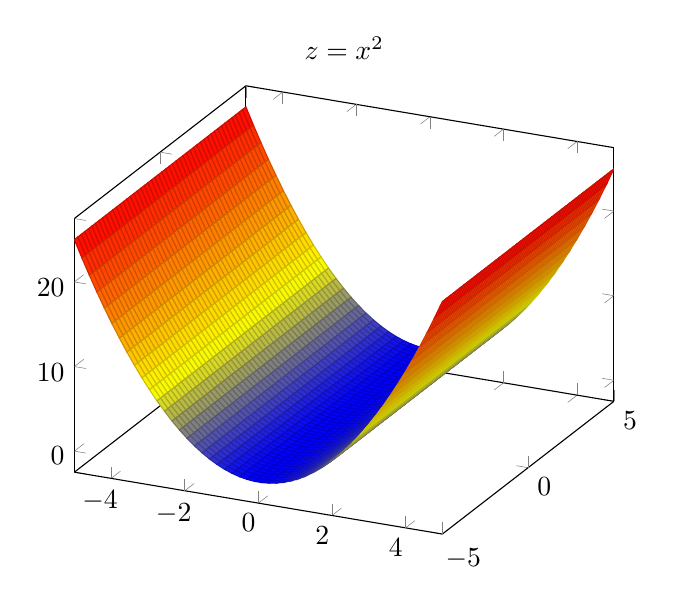
\begin{tikzpicture}
        \begin{axis}[title= \text{$z = x^2$}]
        \addplot3[surf, samples = 50]{x^2};
        \end{axis}
        \end{tikzpicture}
    %Here ends the 2D plot
    \hskip 10pt        
    %Here begins the 2D plot
    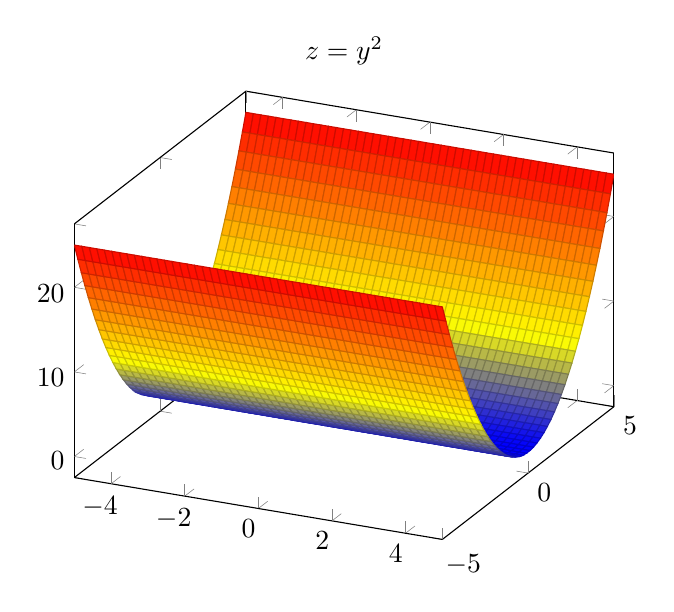
\begin{tikzpicture}
        \begin{axis}[title= \text{$z = y^2$}]
        \addplot3[surf, samples = 50]{y^2};
        \end{axis}
        \end{tikzpicture}
    \vfill
    \vspace{10pt}
\centerline{\bf Thành phố Hồ Chí Minh - 5/10/2023}
\vspace{1cm}
\end{titlepage}

\onehalfspacing
\newpage
\section*{CHỦ ĐỀ 1 - SỐ HỌC (SỐ \& CHỮ SỐ)}
\begin{enumerate}[label=\alph*.]
\item[\textbf{Bài 1.}] Cho $N= 7 + 77 + 777 + 7777 + ... + 77..77$ (có 2018 số hạng) và $M= 3 + 33 + 333 + 3333 + ... + 33..33$ (có 2017 số hạng). Tìm ba chữ số tận cùng của M.N.
\item[\textbf{Bài 2.}] Tìm tổng các chữ số của số $43^7$.
\item[\textbf{Bài 3.}] Tính tổng tất cả các số tự nhiên có 3 chữ số sao cho $\overline{abc}$ với $\overline{abc} = c^5 + 20(a+b+c)$
\item[\textbf{Bài 4.}] Tính tổng sau $\Big \lbrack \sqrt{2} \Big \rbrack + \Big \lbrack \sqrt{3} \Big \rbrack + \Big \lbrack \sqrt{4} \Big \rbrack + \ldots + \Big \lbrack \sqrt{2018} \Big \rbrack + \Big \lbrack \sqrt{2019} \Big \rbrack$ ở đây $\Big \lbrack \sqrt{x} \Big \rbrack$ là số nguyên lớn nhất không vượt quá $x$
\item[\textbf{Bài 5.}] Tìm số tự nhiên $n$ nhỏ nhất biết $n^2$ có hai chữ số đầu là 98 và hai chữ số cuối là 89.
\item[\textbf{Bài 6.}] Tìm số tự nhiên nhỏ nhất mà lập phương của nó có tận cùng là bốn chữ số 8.
\item[\textbf{Bài 7.}] Tìm số tự nhiên nhỏ nhất mà lập phương của nó có tận cùng là 0824.
\item[\textbf{Bài 8.}] Tìm tất cả các số nguyên n sao cho $n + 1930$ và $n + 2539$ đều là số chính phương.
\item[\textbf{Bài 9.}] Gọi $a,b$ là hai chữ số tận cùng của số $A = 2^{15} + 2^{16} + \ldots + 2^{99} + 2^{100}.$ Tính $a^2 + b^2$.
\item[\textbf{Bài 10.}] Tìm chữ số tận cùng của $2019^{2018}$ .
\item[\textbf{Bài 11.}] Tìm số nguyên dương nhỏ nhát có ba chữ số là $\overline{abc}$ sao cho $\overline{abc} = a^3 + b^3 + c^3$. Có còn số nguyên nào thỏa mãn điều kiện trên nữa không? Nêu sơ lược cách tìm.
\item[\textbf{Bài 12.}] Tìm tất cả các số có 6 chữ số thỏa mãn hai tính chất sau:
\begin{enumerate}
    \item[1] Số tạo thành bởi ba chữ số cuối lớn hơn số tạo thành bởi ba chữ số đầu 1 đơn vị.
    \item[2] Là số chính phương.
\end{enumerate}
\item[\textbf{Bài 13.}] Tính giá trị biểu thức
\begin{center}
    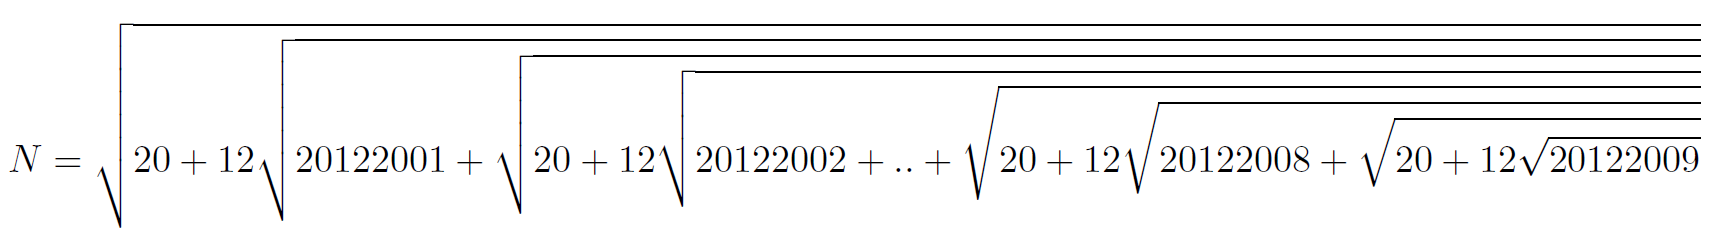
\includegraphics[scale=0.4]{Screenshot 2023-10-07 142830.png}
\end{center}
\item[\textbf{Bài 14.}] Tìm số tự nhiên n nhỏ nhất sao cho khi bình phương số đó ta được số tự nhiên có dạng: 
$$    \overline{2009...2009}   $$
\item[\textbf{Bài 15.}] Tìm một số tự nhiên $x$ biết $x^2$ có bốn chữ số tận cùng 2009 và bốn chữ số đầu tiên cũng là 2009. 
\item[\textbf{Bài 16.}] Tìm ước nguyên tố lớn nhất của số $215^2 + 314^2$.
\item[\textbf{Bài 17.}] Tìm các số lớn nhất và nhỏ nhất trong các số tự nhiên có dạng $\overline{1x2y3z4}$ mà chia hết cho 13.
\end{enumerate}
\newpage
%---------------------------------------------------------
\section*{CHỦ ĐỀ 2 - SỐ HỌC (PHÉP CHIA HẾT \& CHIA ĐỒNG DƯ)}
\begin{enumerate}
\item[\textbf{Bài 18.}] Tìm dư khi chia số $(2+\sqrt{3})^{25} + (2-\sqrt{3})^{25}$ cho 2017.
\item[\textbf{Bài 19.}] Tìm dư khi chia số $(2+\sqrt{3})^{24} + (2-\sqrt{3})^{24}$ cho 2017.
\item[\textbf{Bài 20.}] Tìm dư khi chia số $(4+\sqrt{5})^{25} + (4-\sqrt{5})^{25}$ cho 2018.
\item[\textbf{Bài 21.}] Tìm dư khi chia số $(2+\sqrt{3})^{27} + (2-\sqrt{3})^{27}$ cho 2019.
\item[\textbf{Bài 22.}] Tính tổng các ước lẻ của số 722311901.
\item[\textbf{Bài 23.}] Tìm số tự nhiên $Q$ lớn nhất sao cho khi chia các số $A=8381947$; $B=83814526$; $C=838147105$ cho $Q$ thì ta được cùng một số dư.
\item[\textbf{Bài 24.}] Tìm số chính phương có ba chữ số biết rằng khi chia số đó cho tổng các chữ số của nó thì được thương là 64 và dư là 9.
\item[\textbf{Bài 25.}] Tìm số tự nhiên $x$ nhỏ nhất có 11 chữ số, biết $x$ chia cho 19 dư 17, chia cho 23 dư 1 và chia cho 41 dư 35.
\item[\textbf{Bài 26.}] Tìm số tự nhiên $n$ biết $1563690744^n$ có 14357520 ước số dương.
\item[\textbf{Bài 27.}] Tìm ƯCLN của 40096920, 9474372 và 51135438.
\item[\textbf{Bài 28.}] Tính chính xác ƯCLN và BCNN của hai số $a=24614205$ và $b=10719433$.
\item[\textbf{Bài 29.}] Tìm số dư của phép chia $176594^{29}$ cho 293.
\item[\textbf{Bài 30.}] Tìm số dư của phép chia 24728303034986074 cho 2006.
\item[\textbf{Bài 30*.}] Tìm dư của phép chia $234567891^{12}$ cho $123456789$. (đs: 54306099)
\item[\textbf{Bài 30**}] (chủ đề 1) Tìm một số tự nhiên có 4 chữ số biết rằng nó là một số chính phương và nếu ta thêm vào mỗi chữ số của nó một đơn vị thì cũng được một số chính phương.
\[\begin{cases}\overline{abcd} & =x^{2}\\\overline{(a+1)(b+1)(c+1)(d+1)} & =y^{2}\end{cases}\]
\item[\textbf{Bài 30***}] Tìm tất cả các số tự nhiên $n$ trong khoảng $(1000;10000000)$ sao cho $B = \sqrt[4]{22122010+ 6n}$ là một số tự nhiên. (Trích Đề thi Giải toán trên máy tính cầm tay Quốc gia năm 2013)
\end{enumerate}
\newpage
%---------------------------------------------------------
\section*{CHỦ ĐỀ 3 - ĐA THỨC}
\begin{enumerate}
\item[\textbf{Bài 31.}] Cho biết $\dfrac{210}{5689}=\dfrac{1}{x + \dfrac{1}{y + \dfrac{1}{z}}}$ với $x,y,z$ là các số tự nhiên. \\
Tính giá trị của biểu thức $A = (x-y)(y-z)(z-x)$.
\item[\textbf{Bài 32.}] Tính giá trị của biếu thức $2x^4 - 5x^3 - 10x^2 + 14x + 13$ biết $\dfrac{x+1}{x^2 - x + 1} = \dfrac{1}{2}.$
\item[\textbf{Bài 33.}] Cho $P(x)$ là một đa thức bậc bốn thỏa mãn các điều kiện sau: $P(x)$ chia cho $(x^2+1)$ dư $2x-1$; $P(x)$ chia cho $(x^2+2)$ dư $3x-1$ và $P(1)=2015$. Tính $P(3)$.
\item[\textbf{Bài 34.}] Cho $P(x)$ là một đa thức bậc ba có $P(1) = \dfrac{1}{2}$, $P(2) = \dfrac{2}{3}$, $P(3) = \dfrac{3}{4}$, $P(4) = \dfrac{4}{5}$. Tính chính xác giá trị của $P(39)$.
\item[\textbf{Bài 35.}] Cho $P(x)$ là một đa thức bậc ba có $P(1) = \dfrac{1}{2}$, $P(2) = \dfrac{2}{3}$, $P(3) = \dfrac{3}{4}$, $P(4) = \dfrac{4}{5}$. Tính chính xác giá trị của $P(49)$.
\item[\textbf{Bài 36.}] Cho $P(x)$ là một đa thức bậc bốn thỏa mãn các điều kiện sau: $P(x)$ chia hết cho $(x^2 - 1)$; $P(x)$ chia cho $(x^2 + 2)$ dư $3x-1971$ và $P(2) = 2019$. Tính $P(5)$.
\item[\textbf{Bài 37.}] Cho đa thức bậc ba $f(x)$ sao cho $f(x)$ chia cho $(x^2 + 2)$ dư $2x-1$; $f(x)$ chia cho $(x^2 + x)$ dư $16x-11$. Tính $f(2019).$
\item[\textbf{Bài 38.}] Cho đa thức $P(x)$ có tất cả các hệ số đều là số tự nhiên nhỏ hơn 5, thỏa mãn điều kiện $P(5) = 259$. Tính $P(2019)$
\item[\textbf{Bài 39.}] Cho đa thức bậc ba $P(x)$ sao cho $P(x)$ chia cho $x^2 + 1$ dư $2x-3$, $P(x)$ chia cho $x^2 - 2x$ dư $-3x+2$. Tính $P(2019)$.
\item[\textbf{Bài 40.}] Xác định các hệ số $a,b,c$ của hàm số $f(x) = ax^3 + bx^2 +cx - 2007$. Biết rằng $f(x)$ chia cho $x-16$ có số dư là 29938 và chia cho $x^2 \pm 10x + 24$ có biểu thức số dư là $\dfrac{10873}{16}x-5770.$
%------- CÓ GÌ COI LẠI ĐỀ BÀI VÌ NÓ HƠI MỜ-------------------------------
\item[\textbf{Bài 41.}] Cho đa thức $f(x)$ bậc ba với hệ số của $x^3$ là $k$, $k$ nguyên dương thỏa mãn: $f(2009) = 2010$; $f(2010) = 2011$. Chứng minh rằng $f(2011) - f(2008)$ là số lẻ.
\item[\textbf{Bài 42.}] Cho đa thức $P(x) = (1+x) + 2(1+x)^2 + 3(1+x)^3 + ... + 15(1+x)^{15}$. Được viết dưới dạng $P(x) = a_0 + a_1x + a_2x^2 +...+a_{15}x^{15}$. Tìm hệ số $a_{10}$.
\item[\textbf{Bài 43.}] Cho đa thức $P(x) = x^5 + ax^4 + bx^3 + cx^2 + dx + e.$ Biết rằng $P(1) = 8$, $P(2) = 18$, $P(3) = 32$, $P(4) = 50$, $P(5) = 72$. Tính $P(30)$.
\item[\textbf{Bài 44.}] Biết $P(x)$ là một đa thức bậc bốn, có hệ số của $x^4$ bằng 1 và $P(x)$ chia cho các nhị thức $x+1$, $x+2$, $x-1$, $x-2$ lần lượt có dư là -2, 4, -11, 6.
\begin{enumerate}
    \item[1] Hãy tìm đa thức $P(x)$.
    \item[2] Tính $P(500) + P(200)$. 
\end{enumerate}
\end{enumerate}
\newpage
%-------------------------------------------------------------
\section*{CHỦ ĐỀ 4 - HÀM SỐ \& ĐỒ THỊ HÀM SỐ}
\textbf{LƯU Ý:} tất cả các bài tính khoảng cách hai điểm trong chủ đề này đều phải \textit{chính xác đến 4 chữ số thập phân sau dấu phẩy}.
\begin{enumerate}
\item[\textbf{Bài 45.}] Gọi $M$ là điểm nằm trên $(P):y=x^2$ và $N$ là điểm nằm trên $(P'):y=-\dfrac{1}{2}(x-1)^2$. Tìm giá trị nhỏ nhất của đoạn $MN$.
\item[\textbf{Bài 46.}] Gọi $M$ là điểm nẳm trên parabol $(P):y=x^2-4x+3$ và $N$ là điểm nằm trên đường tròn $(C):(x-6)^2 + (y+1)^2 =1$. Tìm giá trị nhỏ nhất của đoạn MN.
\item[\textbf{Bài 47.}] GỌi $M$ là điểm nằm trên parabol $(P_1):y=x^2-4x+3$ và $N$ là điểm nằm trên parabol $(P_2):y=-(x-5)^2$. Tìm giá trị nhỏ nhất của đoạn MN. 
\item[\textbf{Bài 48.}] Trong hệ trục $Oxy$, parabol $(P):y = x^2 - x - 1$ cắt đường tròn $(C):x^2 + y^2 - 3x + y + 2 = 0$ tại hai điểm $A$ và $B$. Tính độ dài đoạn $AB$.
\item[\textbf{Bài 49.}] Biết đồ thị các hàm số $y = 3^x$ và $y = 11 - 4^{\frac{1}{x}}$ cắt nhau tại 2 điểm $A$ và $B$. Tính khoảng cách giữa $A$ và $B$.
\item[\textbf{Bài 50.}] Cho hàm số $y=f(x)=\dfrac{2x^2 - 5x + 3}{3x^2 - x - 1}$. Tính khoảng cách giữa hai điểm cực trị của đồ thị hàm số đã cho.
\item[\textbf{Bài 51.}] Tính gần đúng hoành độ giao điểm cực trị của đồ thị hàm số đã cho:
\begin{equation*}
(C_1): y = f(x) = 2x^3 - x^2 - 3x -1 \quad \text{ và } \quad (C_2): y = g(x) = \sqrt[3]{x^2 + 2} - \sqrt[3]{2x^3 - 3x + 1}.
\end{equation*}
\item[\textbf{Bài 52.}] Cho hàm số $y=f(x)=2x^3-3(a+3)x^2+18ax-8$. Tìm $a$ để đồ thị hàm số tiếp xúc với trục hoành. 
\item[\textbf{Bài 53.}] Tìm điểm $M$ trên đồ thị của hàm số $y = \dfrac{x^2 + 2x + 3}{4x + 5}$ cách đều hai trục tọa độ.
\item[\textbf{Bài 54.}] Cho điểm $A$ nằm tùy ý trên elip $(E): \dfrac{x^2}{16} + \dfrac{y^2}{9} = 1$ và điểm $B$ nằm tùy ý trên đường thẳng $5x-7y+35=0.$ Tìm giá trị nhỏ nhất của độ dài đoạn thẳng $AB$.
\item[\textbf{Bài 55.}] Đường tròn $x^2 + y^2 + ax + by + c = 0$ đi qua ba điểm $A(5;2),B(3;-4),C(4;7)$. Tính giá trị của $abc$.
\item[\textbf{Bài 56.}] Tính gần đúng tọa độ giao điểm của đường thẳng $(d)$ đi qua hai điểm $A(1;2), B(-3;5)$ và đồ thị $(C)$ hàm số $y = \dfrac{x-1}{3x+7}$.
\item[\textbf{Bài 57.}] Cho parabol $y=ax^2 + bx + c$ đi qua các điểm $A(1;3),B(-2;6),C(-3;-5)$ và đường thẳng $y =(m+1)x + m^2 + 2.$
\begin{enumerate}
\item[a.] Tìm tọa độ các giao điểm của $(P)$ với đường thẳng khi $m=1$.
\item[b.] Tìm tất cả các giá trị của $m$ sao cho $(P)$ và đường thẳng có điểm chung. 
\end{enumerate}
\end{enumerate}
%------------------------------------------------------------
\section*{CHỦ ĐỀ 5 - HÀM SỐ \& GIÁ TRỊ LỚN NHẤT, NHỎ NHẤT}
\begin{enumerate}
\item[\textbf{Bài 58.}] Tính (\textit{chính xác đến 4 chữ số thập phân sau dấu phẩy}) giá trị lớn nhất và giá trị nhỏ nhất của hàm số $f(x) = \dfrac{x\sqrt{3x-1}}{x-3}$ trên $\lbrack 4;12 \rbrack$.
\item[\textbf{Bài 59.}] Tính giá trị nhỏ nhất (\textit{chính xác đến 4 chữ số thập phân sau dấu phẩy}) của biểu thức:
\begin{equation*}
    A = \sqrt{2.3x^2 - \big(\sqrt{5} + 0,4\big)x + \big(4 + 3\sqrt{2}\big)^2}
\end{equation*}
\item[\textbf{Bài 60.}] Tính gần đúng (\textit{chính xác đến 4 chữ số thập phân sau dấu phẩy}) giá trị lớn nhất và giá trị nhỏ nhất của biểu thức $A = \dfrac{2,3x^2 - 3,4x + 5,6}{0,3x^2 + 1,9}$.
\item[\textbf{Bài 61.}] Tính gần đúng (\textit{chính xác đến 4 chữ số thập phân sau dấu phẩy}) giá trị lớn nhất của biểu thức $p = \dfrac{\sqrt{3,7x - 8,2}}{1,2x + 2,3}.$ 
\item[\textbf{Bài 62.}] Tính gần đúng (\textit{chính xác đến 4 chữ số thập phân sau dấu phẩy}) giá trị lớn nhất của hàm số $y = \dfrac{\sqrt{2,3x - 2,7}}{1,3x + 3,4}.$ 
\item[\textbf{Bài 63.}] Cho hai số tự nhiên $x,y$ thỏa mãn $y^3 = x^3 + 2x^2y + 11xy + 11x^2$. Biết $y$ có hai chữ số. tìm giá trị lớn nhất của $y$. 
\item[\textbf{Bài 64.}] Tính (\textit{chính xác đến 4 chữ số thập phân sau dấu phẩy}) giá trị lớn nhất và giá trị nhỏ nhất của hàm số $f(x) = \dfrac{x\ln x}{x+1}$ trên $\bigg\lbrack \dfrac{1}{4};2 \bigg\rbrack$.
\item[\textbf{Bài 65.}] Cho các hàm số $f(x) = 2008x^{-5} - 3x + 2009\sqrt{x^2 + 2007} \thickspace (x \neq 0).$ Tính các giá trị sau $f(1); f(\sqrt{2}); f(\sqrt{2009}); f(\sqrt{2008\sqrt{2009}}); f(\sqrt{2006 + 18\sqrt{2023}})$.
\item[\textbf{Bài 66.}] Tính gần đúng giá trị lớn nhất và nhỏ nhất của hàm số: $y = \dfrac{2\sin x + 3\cos x - 1}{\cos x + 2}.$
\item[\textbf{Bài 67.}] Cho các hàm số $f(x) = \dfrac{2x^2 + 3x - 5}{x^2 + 1};\thickspace g(x) = \dfrac{2\sin x}{1+\cos^4 x}.$ Hãy tính giá trị của các hàm hợp $g(f(x)), f(g(x)), f(f(x)), g(g(x))$ tại $x = \sqrt[3]{5}$.
\item[\textbf{Bài 68.}] Cho hàm số: $f(x) = \dfrac{\sqrt[3]{x} + 3^{\sqrt{x}}}{\log^2_3 x + 12}$. Tính tổng: $S = f(\cot^2 1) + f(\cot^2 2) + ... + f(\cot^2 20).$
\item[\textbf{Bài 69.}] Tính gần đúng giá trị lớn nhất và nhỏ nhất của hàm số: $f(x) = \dfrac{2^{\cos 2x} + (x^2 +1).\sin x + 3}{x^2 - x + 1}$ trên $\lbrack 0;1 \rbrack$.
\item[\textbf{Bài 70.}] Cho hàm số $y = 24x - \cos 12x - 3\sin 8x.$ Tìm giá trị lớn nhất của hàm số trên $\bigg\lbrack -\dfrac{\pi}{6};\dfrac{\pi}{6} \bigg\rbrack$.
\item[\textbf{Bài 71.}] Tìm giá trị lớn nhất và giá trị nhỏ nhất của hàm số: $y = f(x) = \dfrac{2\sin x +3\cos x - 1}{\sin x + 2}$.
\item[\textbf{Bài 72.}] Cho hàm số $f(x) = \dfrac{2\sqrt{\log (x^2 + 1) + 3}}{2^{\log x} + 1}$. Tính giá trị của tổng $S = f(1) + f(2) + ... + f(100).$
\item[\textbf{Bài 73.}] Tính gần đúng giá trị nhỏ nhất, giá trị lớn nhất của hàm số $y = 3x + 5\cos 2x$ trên đoạn $\lbrack 0;\pi \rbrack$.
\item[\textbf{Bài 74.}] Tìm GTNN và GTLN của hàm số $y = \sqrt{x-1} + \sqrt{5-2x}$.
\item[\textbf{Bài 75.}] Cho hàm số $f(x) = \dfrac{x^3}{6\sqrt{x^3} + \sqrt{3}}$. Tính tổng $S = f(1) + f(2) + ... + f(100).$
\end{enumerate}
%-----------------------------------------------------------------
\section*{CHỦ ĐỀ 6 - ĐẠI SỐ (PHƯƠNG TRÌNH \& HỆ PHƯƠNG TRÌNH)}
\begin{enumerate}
\item[\textbf{Bài 76.}] Biết phương trình $x^5 +ax^2 + bx - 1 = 0$ có một nghiệm là $x=1-\sqrt{2}$ và $a,b$ đều là những số nguyên. Tính $a^2 + b^2$.
\item[\textbf{Bài 77.}] Tìm nghiệm nguyên dương của phương trình $4x^2(2x+3y^2) + y^4(6x+y+y^2) = 319330$.
\item[\textbf{Bài 78.}] Biết $x_1,x_2,x_3,x_4$ là 4 nghiệm của phương trình $3x^4 - 10x^3 - x^2 + 4x + 1 = 0$. Tính giá trị của biểu thức $S = x^7_1 + x^7_2 + x^7_3 + x^7_4$ (\textit{chính xác đến 4 chữ số thập phân sau dấu phẩy}).
\item[\textbf{Bài 79.}] Tính gần đúng nghiệm của phương trình $7x^2 + 8y^2 = 2360$.
\item[\textbf{Bài 80.}] Tìm các số nguyên dương $x,y$ sao cho $x^2 + 2y^2 = 2009$.
\item[\textbf{Bài 81.}] Tính gần đúng các nghiệm của hệ phương trình: $\begin{cases}
    x^3 + y^3 = 6 + xy \\
    x^2 + y^2 + x + y = 5
\end{cases}$
\item[\textbf{Bài 81*.}] Giải phương trình sau:  
$$x\left(\sqrt{3-2x + \sqrt{5(1-x^2)} + \sqrt{\frac{3}{2}}} \right) = \sqrt{\frac{2}{3}}$$
\item[\textbf{Bài 81**.}] Giải PT sau: $\log_{5}(x+2) + \log_{3}(x) = \log_{2018}(x+2015) + \log_{2019}(x+2016).$ (đs $x = 3$)
\end{enumerate}
%-----------------------------------------------------------------
\section*{CHỦ ĐỀ 7 - ĐẠI SỐ \& GIẢI TÍCH (PHƯƠNG TRÌNH, HỆ PHƯƠNG TRÌNH)}
\begin{enumerate}
\item[\textbf{Bài 82.}] Tính tổng các nghiệm của phương trình: $10\sin x = x$ trên khoảng $(0;10)$ (\textit{chính xác đến 4 chữ số thập phân sau dấu phẩy}).
\item[\textbf{Bài 83.}] Tính tổng các nghiệm của phương trình: $10\cos x = x$ trên khoảng $(0;10)$ (\textit{chính xác đến 4 chữ số thập phân sau dấu phẩy}).
\item[\textbf{Bài 84.}] Tính gần đúng (\textit{chính xác đến 4 chữ số thập phân sau dấu phẩy}) tổng tất cả các nghiệm thuộc đoạn $[10;20]$ của phương trình: $2\sin x + \sin 3x = 1.$
\item[\textbf{Bài 85.}] Giải phương trình $2^x = 2018x + 2017$ (\textit{chính xác đến 4 chữ số thập phân sau dấu phẩy}).
\item[\textbf{Bài 86.}] Tìm nghiệm gần đúng (độ, phút, giây) của phương trình $\sin^2 2x + 4(\sin x + \cos x) = 3$.
\item[\textbf{Bài 87.}] Cho $s\sin x = 0,3 \thickspace\bigg(0 < x < \dfrac{\prod}{2}\bigg): \cos y = -0,3\thickspace\bigg( \prod < y < \dfrac{3\prod}{2}\bigg)$. Tính gần đúng giá trị của biểu thức sau: $P = \dfrac{\tan^5 (y^2 + 2y^2) + \cot^5 (x^2 - 2y^2)}{\sin^7 (x-y) + \cos^7 (x+y)}.$
\item[\textbf{Bài 88.}] Cho biết $\tan x = \tan 35^0.\tan 36^0.\tan 37^0\ldots\tan 52^0\tan 53^0$ và $0^0 < x < 90^0$. Tính
$$M = \frac{\tan^2 x(1+\cos^3 x) + \cot^2 x(1+\sin^3 x)}{(\cos^3 x + \sin^3 x)(1 + \cos x + \sin x)}$$
\item[\textbf{Bài 89.}] Cho hàm số $y = \dfrac{2x^2 - 7x - 4}{x^2 - 5x + 6}$. Tính $y^{(5)}$ tại $x = \dfrac{3}{5}$.
\item[\textbf{Bài 90.}] Cho phương trình $x + \log_6 (47-6^x) = m$
\begin{enumerate}
\item[a)] Tìm các nghiệm gần đúng của phương trình khi $m = 0,4287$.
\item[b)] Tìm giá trị nguyên lớn nhất của $m$ để phương trình có nghiệm.
\end{enumerate}
\item[\textbf{Bài 91.}] Tính gần đúng nghiệm của phương trình: $\sin x.\sin 2x + \sin 3x = 6\cos^3 x$ (độ, phút, giây).
\item[\textbf{Bài 92.}] Tính gần đúng đạo hàm cấp 30 của hàm số: $f(x) = \sin^2 x$ tại $x = \dfrac{201209\pi}{5}$.
\item[\textbf{Bài 93.}] Tính gần đúng nghiệm (độ, phút, giây) của phương trình:
$$3\sin x - \cos x + 2 = \dfrac{3}{3\sin x - \cos x}$$
\item[\textbf{Bài 94.}] Tính gần đúng nghiệm (độ, phút, giây) của PT: $2\sin^2 x + 9\sin x.\cos x - 4\cos^2 x= 0$
\item[\textbf{Bài 95.}] Tính gần đúng nghiệm (độ, phút, giây) của phương trình:
\begin{enumerate}
\item[a)] $2\sin x - 7\cos x + 4 = 0$, với $270^o < x < 450^o$.
\item[b)] $2(\sin y + \cos y) + \sin y.\cos y + 1 = 0$, với $90^o < x < 360^o$.
\end{enumerate}
\item[\textbf{Bài 96.}] Cho $\tan x = 2$ $(2\pi < x <3\pi)$ và $2\sin y + 3\cos y = 1$ $(0 < y < \pi)$. Tính gần đúng: 
\item[a)] $A = \dfrac{\sin^2 x - \cos^3 x}{2\tan^2 x + 3\cot^4 x}$
\item[b)] $B = \dfrac{\tan^2(x^2 - y) + \cot^2(x-y^2)}{\sin^2(x^2 + y) + \cos^4(x+y^2)}$
\item[\textbf{Bài 97.}] Tính nghiệm thuộc khoảng $(0;2\pi)$ của phương trình $3\cos3x - 4x + 2 = 0$.
\end{enumerate}
\newpage
%------------------------------------------------------------------------------------------------------------------------------------------------------------------------------
\section*{CHỦ ĐỀ 8 - DÃY SỐ \& HỒI QUY}
\begin{enumerate}
\item[\textbf{Bài 98.}] Cho dãy số $(x_n)$ được xác định bởi $x_1 = 1, x_2 = 2, x_n = nx_{n-1}-x_{n-2} \thickspace (n \geq 3)$. Tính (\textit{ghi kết quả chính xác}): $x_{12},x_{13},x_{14},x_{15},\ldots$
\item[\textbf{Bài 99.}] Cho dãy số $(x_n)$ được xác định bởi $x_1 = 1, x_2 = 1, x_n = x_{n-1} - nx_{n-2} + 2n^2 \thickspace (n \geq 3)$. Tính (\textit{ghi kết quả chính xác}): $x_{18},x_{19},x_{20},x_{21},\ldots$
\item[\textbf{Bài 100.}] Cho dãy số $(x_n)$ được xác định bởi $x_1 = 1, x_2 = 2, x_n = -x_{n-1}+x_{n-2}+n^2 \thickspace (n \in \mathbb{N},n \geq 3)$. Tính $x_{32}$.
\item[\textbf{Bài 101.}] Cho hai dãy số $(u_n)$ và $(v_n)$ có: $u_1 =1; v_1 = 2; u_{n+1} = 22v_n - 15u_n; v_{n+1} = 17v_n - 12u_n \thickspace (n \geq 1).$
\begin{enumerate}
\item[a)] Tính $u_5, u_{10}, u_{15}, u_{18}, v_5, v_{10}, v_{15}, v_{18}.$
\item[b)] Lập quy trình bấm phím.
\end{enumerate}
\item[\textbf{Bài 102.}] Cho 2 dãy số $\lbrace u_n \rbrace$ và $\lbrace v_n \rbrace$ 
$\text{ với }\left\{\def\arraystretch{1.2}\begin{tabular}{@{}l@{\quad}l@{}}
  $u_1 = 1; v_1 = 2$ \\
  $u_{n+1} = 22v_n - 15u_n$ \\
  $v_{n+1} = 17v_n - 12u_n$
\end{tabular}\right.$, với $n = 1,2,3,\ldots,k,\ldots$
\begin{enumerate}
    \item[1.] Tính $u_{5},u_{10}, u_{15}, u_{19}, u_{19}, v_{5},v_{10}, v_{15}, v_{19}, v_{19}$
    \item[2.] Viết quy trình ấn phím liên tục của $u_{n+1}$ và $v_{n+1}$ theo $u_n$ và $v_n$.
\end{enumerate}
\item[\textbf{Bài 103.}] Tìm $a_{2009}$ $\text{ biết }\left\{\def\arraystretch{1.2}\begin{tabular}{@{}l@{\quad}l@{}}
  $a_1 = 0$ \\
  $a_{n+1} = \dfrac{n(n+1)}{(n+2)(n+3)}(a_n + 1) \quad n \in \mathbb{N}^*$ 
\end{tabular}\right.$
\item[\textbf{Bài 104.}] Cho dãy số $u_n$ xác định bởi: $u_1 = 1, u_2 = 2, u_3 = 3,\ldots,u_{n+1} = u_n + 2u_{n-1} + 3u_{n-2} \thickspace (n \geq 3)$.
\begin{enumerate}
    \item[1.] Tính giá trị của $u_5, u_5, u_6, u_7$.
    \item[2.] Viết quy trình bấm phím để tính $u_{n+1}$.
    \item[3.] Sử dụng quy rình bấm phím trên để tính $u_{19}, u_{21}, u_{25}, u_{28}$.
\end{enumerate}
\item[\textbf{Bài 105.}] Cho dãy số $(u_n)$ thỏa điều kiện sau:$u_1 = 1, u_2 = -1, u_{n+2} = 2u_{n+1} - 3u_n$. Hãy tính tổng 22 số hạng đầu tiên của dãy số $u_n$.
\item[\textbf{Bài 106.}] Cho $u_1 = 4, u_2 = 7, u_3 = 5 \thickspace \& \thickspace u_n = 2u_{n-1} - u_{n-2} + u_{n-3} \thickspace (4 \leq n \in \mathbb{N})$. Tính $u_{30}$
\item[\textbf{Bài 107.}] Dãy số $\lbrace u_n \rbrace$ được cho bởi công thức: $u_n = n + \dfrac{2006}{n^2},$ với mọi $n$ nguyên dương. Tìm số hạng nhỏ nhất của dãy số.
\item[\textbf{Bài 108.}] Cho dãy số $u_n$ được xác định bởi: $\left\{\def\arraystretch{1.2}\begin{tabular}{@{}l@{\quad}l@{}}
  $u_1 = 2$ \\
  $u_{n+1} = \dfrac{1}{2}(3+u_n)$ 
\end{tabular}\right.$ \\Tính 12 số hạng đầu tiên của dãy đã cho.\\ Tính tổng 20 số hạng đầu của dãy.\\ Viết quy trình bấm phím thực hiện việc tính liên tiếp 20 số hạng đầu và tổng của 20 số hạng đó.
\end{enumerate}
\newpage
%----------------------------------------------------------------------------------------------------------------------------------------------------------------------------------------------------------------------------
\section*{CHỦ ĐỀ 9 - DÃY SỐ \& TỔ HỢP}
\begin{enumerate}
    \item[\textbf{Bài 109.}] Tính gần đúng: $S = \dfrac{1}{2.4.6} + \dfrac{3^2}{4.6.8} + \cdots + \dfrac{2019^2}{2020.2022.2024}$ (\textit{chính xác đến 4 chữ số thập phân sau dấu phẩy}).
    \item[\textbf{Bài 110.}] Tính tổng: $S = \dfrac{1}{2\times3} - \dfrac{2}{3\times4} + \cdots + \dfrac{99}{100\times101} - \dfrac{100}{101\times102}$. Lấy nguyên kết quả hiện trên màn hình.
    \item[\textbf{Bài 111.}] Tính chính xác giá trị phần nguyên và phần thập phân (\textit{ghi dưới dạng phân số tối giản}) của: \[S = \displaystyle \sum_{k=1}^{100} \dfrac{3k^3  + 11k^2 + 5k - 2}{k^2+4k+3}\]
    \item[\textbf{Bài 112.}] Cho biết kết quả của tổng $\displaystyle \sum_{k=1}^{100} \dfrac{k^4 + k^3 - 7k^2 - k + 7}{k^2 + 4k + 3}$ có dạng hỗn số là $A\dfrac{m}{n}$. Tính $A + m^2 - n^3$.
    \item[\textbf{Bài 113.}] Cho biết $\displaystyle \sum_{k=0}^{1000} \dfrac{k^4 + k^3 - 4k^2 - 4k + 10}{k^2 + 3k + 2} = I\dfrac{m}{n}$ là một hỗn số. Tính giá trị $I + m - n^3$.
    \item[\textbf{Bài 114.}] Tìm hệ số của các số hạng chứa $x^4$ và $x^{10}$ trong khai triển nhị thức Newton của $\left( \dfrac{1}{x^3} + \sqrt{x^5}\right)^n$. Biết rằng: $C_{10}^{n+1} - C_{15}^{n} = 7(n+3) \thickspace (n>0)$.
    \item[\textbf{Bài 115.}] Tính giá trị của biểu thức\[\sqrt{1+\dfrac{1}{2}}.\sqrt{1+\dfrac{1}{2}+\dfrac{1}{3}}.\sqrt{1+\dfrac{1}{2}+\dfrac{1}{3}+\dfrac{1}{4}}\cdots\sqrt{1+\dfrac{1}{2}+\dfrac{1}{3}+\dfrac{1}{4} + \cdots + \dfrac{1}{20}}\]
    \item[\textbf{Bài 116.}] Hãy rút gọn công thức: $S_n(x) = 2 + 2.3x + 3.4x^2 + \cdots + n.(n-1)x^{n-2}.$ Tính $S_{17}(-\sqrt{2})$.
    \item[\textbf{Bài 117.}] Tính tổng các hệ số của các số hạng chứa $x^5,x^{10}$ trong khai triển $\left(\sqrt{x} + \dfrac{2}{\sqrt[3]{x}}\right)^{30}.$
    \item[\textbf{Bài 118.}] Tính giá trị của biểu thức sau: $\sqrt{2+\sqrt[3]{3 + \sqrt[4]{4 + \ldots + \sqrt[8]{8 + \sqrt[9]{9}}}}}.$
\end{enumerate}
%--------------------------------------------------------------------------------------------------------------------------------------------------------------------------------------------------------------------------
\section*{CHỦ ĐỀ 10 - ỨNG DỤNG TÍCH PHÂN ĐỂ TÍNH DIỆN TÍCH HÌNH PHẲNG \& THỂ TÍCH KHỐI TRÒN XOAY}
\begin{enumerate}
    \item[\textbf{Bài 119.}] Tính diện tích hình phẳng giới hạn bởi đồ thị các hàm số $y=x^2-3x+3, y = \ln x,y=0$.
    \item[\textbf{Bài 120.}] Gọi $(d)$ là tiếp tuyến của đồ thị hàm số $y = \dfrac{x+1}{\sqrt{4x^2 + 2x + 1}} \thickspace (C)$ tại điểm $M(-1,0)$. Tính diện tích hình phẳng xác định bởi $(d),(C)$ và trục tung (\textit{chính xác đến 4 chữ số thập phân sau dấu phẩy}).
\end{enumerate}
\newpage
%----------------------------------------------------------------------------------------------------------------------------------------------------------------------------------------------------------------------------
\section*{CHỦ ĐỀ 11 - HÌNH HỌC PHẲNG \& HỆ THỨC LƯỢNG TRONG TAM GIÁC ĐƯỜNG TRÒN}
\begin{enumerate}
    \item[\textbf{Bài 121.}] Cho tam giác $ABC$ có $AB = 2,9;\thickspace BC = 4,1;\thickspace CA = 3,6$. Trên các cạnh $AB,BC,CA$ lần lượt lấy các điểm $D,E,F$ sao cho $AD = 1,4;\thickspace BE = 1,8;\thickspace CF = 1,2$. $AE$ cắt $DF$ tại $M$. Tính gần đúng (\textit{chính xác đến 2 chữ số thập phân sau dấu phẩy}): 
        \begin{enumerate}
            \item[a)] Diện tích tam giác $ABC$.
            \item[b)] Bán kính đường tròn ngoại tiếp tam giác $DEF$.
            \item[c)] Độ dài đoạn thẳng $MD$.
        \end{enumerate}
    \item[\textbf{Bài 122.}] Cho tam giác $ABC$ có $AB = 14;\thickspace BC = 15;\thickspace CA = 17$. Hình vuông $MNPQ$ có $M,N$ thuộc cạnh $BC$. $P,Q$ lần lượt thuộc cạnh $AB,AC$. Tính gần đúng (\textit{chính xác đến 2 chữ số thập phân sau dấu phẩy}):
        \begin{enumerate}
            \item[a)] Diện tích hình vuông $MNPQ$.
            \item[b)] Khoảng cách từ $A$ đến tâm $O$ của hình vuông $MNPQ$.
        \end{enumerate}
    \item[\textbf{Bài 123.}] Cho tam giác $ABC$ có $AB = 5,7;\thickspace BC = 8,3;\thickspace CA = 7,6$. Đường trung tuyến $AM$ cắt phân giác $BD$ tại $I$. Tính (\textit{chính xác đến 2 chữ số thập phân sau dấu phẩy}):
        \begin{enumerate}
            \item[a)] $IA,IB,IC$.
            \item[b)] Bán kính $R$ của đường tròn ngoại tiếp tam giác $CDM$.
            \item[c)] Bán kính $r$ của đường tròn nội tiếp tam giác $CDM$.
            \item[d)] Diện tích $S$ của tứ giác $CDIM$.
        \end{enumerate}
    \item[\textbf{Bài 124.}] Cho tam giác $ABC$ có các góc $A,C$ nhọn; $BC = 3,5$; đường cao $BH = 2,7$ và bán kính đường tròn ngoại tiếp bằng $2,8$. Gọi $K$ là giao điểm của $BH$ và trung tuyến $AM$. Tính (\textit{chính xác đến 2 chữ số thập phân sau dấu phẩy}):
        \begin{enumerate}
            \item[a)] Độ dài các cạnh $AB,AC$ và trung tuyến $AM$ của tam giác $ABC$.
            \item[b)] Bán kính $R$ của đường tròn ngoại tiếp tam giác $ABC$.
            \item[c)] Diện tích $S$ của tứ giác $CHKM$.
        \end{enumerate}
    \item[\textbf{Bài 125.}] Cho tam giác $ABC$ cân tại $A$ và nội tiếp trong đường tròn bán kính $R = 2019$. Tính gần đúng (\textit{chính xác đến 4 chữ số thập phân sau dấu phẩy}) giá trị lớn nhất của đường cao $BH$.
    \item[\textbf{Bài 126.}] Cho tam giác $ABC$ có đường cao $BH;\thickspace AB = 3,7;\thickspace AC = 4,9;\thickspace BC = 5,3$. Trên cạnh $BC$ lấy điểm $M$ sao cho $MC = 2MB$. Gọi $I$ là giao điểm của $AM$ và $BH$. Tính gần đúng (\textit{chính xác đến 2 chữ số thập phân sau dấu phẩy}) độ dài các đoạn $IA,IB$; bán kính $R$ của đường tròn ngoại tiếp tam giác $IBM$; bán kính $r$ của đường trong nội tiếp tam giác $IBM$.
    \item[\textbf{bài 127.}] Cho tam giác $ABC$ cân tại $A$ và nội tiếp trong đường tròn bán kính $R = 2006$. Tính giá trị lớn nhất của đường cao $BH$.
    \item[\textbf{Bài 128.}] Tính gần đúng diện tích phần chung của hai đường tròn có bán kính $6cm$ và $7cm$, biết khoảng cách giữa hai tâm của chúng bằng $8cm$.
    \item[\textbf{Bài 129.}] Cho tam giác vuông với các cạnh bên có độ dài là $\sqrt[4]{3}$ và $\sqrt[3]{4}$, hãy tính tổng các bình phương của các trung tuyến.
\end{enumerate}
%-----------------------------------------------------------------------------------------------------------------------------------------------------------------------------------------------------
\section*{CHỦ ĐỀ 12 - HÌNH HỌC PHẲNG GẮN TỌA ĐỘ OXY}
\begin{enumerate}
    \item[\textbf{Bài 130.}] Cho tam giác $ABC$ vuông tại đỉnh $A(-1;3)$ cố dịnh, còn các đỉnh $B$ và $C$ di chuyển trên đường thẳng đi qua 2 điểm $M(-3;-1),\thickspace N(4;4)$. Biết rằng $\widehat{ABC} = 30^o$. Hãy tính tọa độ điểm $B$.
    \item[\textbf{Bài 131.}] Cho tam giác $ABC$ có các đỉnh $A(9;-3),\thickspace B\left(\dfrac{3}{7};-\dfrac{1}{7}\right)$ và $C(-1;7)$.
        \begin{enumerate}
            \item Viết phương trình đường tròn ngoại tiếp tam giác $ABC$.
            \item Viết phương trình tiếp tuyến của đường tròn, biết tiếp tuyến đi qua điểm $M(-4;1)$.
        \end{enumerate}
    \item[\textbf{Bài 132.}] Tính gần đúng giá trị của $a$ và $b$ nếu đường thẳng $y=ax+b$ đi qua điểm $A(5;2)$ và là tiếp tuyến của Elip $\dfrac{x^2}{16} + \dfrac{y^2}{9} = 1$.
    \item[\textbf{Bài 133.}] Trong mặt phẳng với hệ tọa độ Oxy, cho tam giác $ABC$ biết $A(2;-4),\thickspace B(-4;-1),\thickspace C(6;4).$ Gọi $D$ và $E$ là chân đường các đường phân giác góc $A$ trên đường thẳng $BC$. Tính diện tích tam giác $ADE$.
    \item[\textbf{Bài 134.}] Cho tứ giác $ABCD$ có $A(10;1)$, $B$ nằm trên trục hoành, $C(1;5)$. $A$ và $C$ đối xứng nhau qua $BD$, $M$ là giao điểm của hai đường chéo $AC$ và $BD$; $BM=\dfrac{1}{4}BD$
        \begin{enumerate}
            \item Tính diện tích tứ giác $ABCD$.
            \item Tính độ dài đường cao đi qua đỉnh $D$ của tam giác $ABD$.
        \end{enumerate}
    \item[\textbf{Bài 135.}] Cho tam giác $ABC$, $E$ là trung điểm của $BC$, trên cạnh $AC$ lấy điểm $D$ sao cho $AD=3DC$. Tính số đo (độ, phút, giây) các góc $BCA$ và $EAC$.
\end{enumerate}
%----------------------------------------------------------------------------------------------------------------------------------------------------------------------------------------------------------------
\section*{CHỦ ĐỀ 13 - HÌNH HỌC KHÔNG GIAN }
\subsection*{KHỐI ĐA DIỆN}
\begin{enumerate}
    \item[\textbf{Bài 136.}] Cho tam giác $BCD$ có $BD = 4,5;\thickspace DC = 6,3;\thickspace CB = 3,7$; trọng tâm $G$. Trên đường thẳng vuông góc với mp $(BCD)$ tại $G$ lấy điểm $A$ sao cho $GA = 6$. Tính gần đúng (\textit{chính xác đến 2 chữ số thập phân sau dấu phẩy})
        \begin{enumerate}
            \item Độ dài các cạnh $AB,\thickspace AC,\thickspace AD$.
            \item Chiều cao $BK$ của tứ diện $ABCD$.
            \item Bán kính $R$ của mặt cầu ngoại tiếp tứ diện $ABCD$.
        \end{enumerate}
    \item[\textbf{Bài 137.}] Cho tam giác $ABC$ có $AB = 3,5;\thickspace BC = 5,3;\thickspace CA = 4,8$. Gọi $M$ là trung điểm của $AC$, $N$ là điểm trên cạnh $BC$ sao cho $BC = 3BN$ và $BM$ cắt $AN$ tại I. Trên đường thẳng vuông góc với mp $(ABC)$ tại $I$, lấy điểm $S$ sao cho $SI = 7$. Tính gần đúng (\textit{chính xác đến 2 chữ số thập phân sau dấu phẩy}):
        \begin{enumerate}
            \item Độ dài các cạnh $SA,\thickspace SB,\thickspace SC$ của tứ diện $S.ABC$.
            \item Chiều cao $BK$ của tứ diện $S.ABC$.
            \item Bán kính $R$ của mặt cầu ngoại tiếp tứ diện $S.ABC$.
        \end{enumerate}
    \item[\textbf{Bài 138.}] Cho tứ diện $ABCD$ có $AD=BC=6;\thickspace AB=CD=5;\thickspace AC=DB=7.$ Tính khoảng cách $d$ giữa $AD$ và $BC$.
    \item[\textbf{Bài 139.}] Cho tam giác $BCD$ có $BD = 5;\thickspace BD = 7; \thickspace CB = 8$; trọng tâm $G$. Trên đường thẳng vuông góc với mp $(BCD)$ tại $G$, lấy điểm $A$ sao cho $GA = 6$ .Tính gần đúng (\textit{chính xác đến 2 chữ số thập phân sau dấu phẩy}):
        \begin{enumerate}
            \item Độ dài các cạnh $AB,AC,AD$.
            \item Chiều cao $BK$ của tứ diện $ABCD$.
        \end{enumerate}
    \item[\textbf{Bài 140.}] Tính thể tích của một khối đa diện 12 mặt đều, mỗi mặt là một ngũ giác đều cạnh bằng $1cm$ (\textit{chính xác đến 2 chữ số thập phân sau dấu phẩy}).
    \item[\textbf{Bài 141.}] Người ta cắt một tờ giấy hình vuông cạnh bằng 1 để gấp thành một hình chóp tứ giác đều sao cho bốn đỉnh của hình vuông dán lại thành đỉnh của hình chóp. Tính cạnh đáy của khối chóp để thể tích lớn nhất.
    \item[\textbf{Bài 142.}] Cho tứ diện $ABCD$ có các cạnh $AB = 7\sqrt{2}, BC = 6\sqrt{2}, CD = 5\sqrt{2}, BD = 4\sqrt{2}$ và chân đường vuông góc hạ từ $A$ xuống mặt phẳng $(BCD)$ là trọng tâm của tam giác $BCD$. Tính $V_{ABCD}$.
    \item[\textbf{Bài 143.}] Cho hình chóp $S.ABCD$ có đáy $ABCD$ là hình chữ nhật. $SA$ vuông góc với đáy và $AB = 3,54cm; AD = 4,35cm; SA = 5,22cm.$ Lấy các điểm $B',D'$ theo thứ tự thuộc $SB,SD$ sao cho $AB'$ vuông góc với $SB$, $AD'$ vuông góc với $SD$. Mặt phẳng $(AB'D')$ cắt $SC$ tại $C'$. Tính thể tích khối chóp $S.AB'C'D'$.
    \item[\textbf{Bài 144.}] Cho tứ diện $ABCD$ có $AB=1cm, AC = 2cm, AD = 5cm$ và 
        \[\angle BAC = \frac{2}{3}\angle CAD = \frac{1}{2}\angle BAD = 40^o\]
    Tính giá trị gần đúng thể tích của khối tứ diện $ABCD$.
    \item[\textbf{Bài 145.}] Cho hình chóp $S.ABCD$ có $SA$ vuông góc với đáy, đáy $ABC$ là tam giác cân tại $A$ có trung tuyến $AD = 5cm$. Cạnh $SB$ tạo với đáy một góc $45^o$ và tạo với mặt phẳng $(SAD)$ một góc $15^o$. Tính cạnh $SB$.
    \item[\textbf{Bài 146.}] Cho hình chóp thập diện đều có đáy nội tiếp trong đường tròn bán kính $r = 3,5cm$, chiều cao $h = 8cm$. Tính diện tích xung quanh của hình chóp và thể tích của khối chóp.
\end{enumerate}
\subsection*{KHỐI TRÒN XOAY}
\begin{enumerate}
    \item[\textbf{Bài 147.}] Một người thợ làm cái chum từ một khối cầu có bán kính $5,61dm$ bằng cách cắt bỏ hai chỏm cầu đối nhau. Tính thể tích của cái chum biết chiều cao của nó bằng $6,25dm$ (\textit{chính xác đến 2 chữ số thập phân sau dấu phẩy}) và bỏ qua độ dày của chum.
    \item[\textbf{Bài 148.}] Khi sản xuất vỏ lon sữa bò hình trụ, các nhà thiết kế luôn đặt mục tiêu sao cho chi phí nguyên liệu làm vỏ hộp (sắt tây) là ít nhất. Tức là diện tích toàn phần của hình trụ là nhỏ nhất. Hãy cho biết diện tích toàn phần của lon khi ta muốn có thể tích của lon là $314cm^3$.
\end{enumerate}
\section*{CHỦ ĐỀ 14 - TOÁN THỰC TẾ}
\begin{enumerate}
    \item[\textbf{Bài 149.}] Sự tăng trưởng của một loại vi khuẩn theo công thức $S = Ae^{rt}$ trong đó $A$ là số lượng vi khuẩn ban đầu, $r$ là tỉ lệ tăng trưởng, $t$ là thời gian tăng trưởng. Biết rẳng số lượn vi khuẩn ban đầu là $100$ con và sau $5$ giờ có $500$ con. Hỏi sau thời gian bao lâu thì số lượng vi khuẩn tăng gấp $10$ lần so với số lượng ban đầu.
    \item[\textbf{Bài 150.}] Một người được lĩnh lương khỏi điểm là $700.000$ đ/tháng. Cứ ba năm anh ta lại được tăng lương thêm $7\%$. Hỏi sau $30$ năm làm việc anh ta được lĩnh tất cả bao nhiêu tiền (Lấy chính xác đến hàng đơn vị).
    \item[\textbf{Bài 151.}] Tính diện tích phần gạch chéo (được giới hạn trong 4 cung tròn như hình vẽ), biết $ABCD$ là hình vuông cạnh $5,35cm$; $M,N,P,Q$ lần lượt là trung điểm của $AB,BC,CD,DA$.
    \begin{center}
        \definecolor{ffffff}{rgb}{1,1,1}
\definecolor{uuuuuu}{rgb}{0.26666666666666666,0.26666666666666666,0.26666666666666666}
\definecolor{ududff}{rgb}{0.30196078431372547,0.30196078431372547,1}
\begin{tikzpicture}[line cap=round,line join=round,>=triangle 45,x=1cm,y=1cm]
\clip(-2.22356185913537,-2.333894329186131) rectangle (2.288980221535642,2.631603798887524);
\fill[line width=2pt,fill=black,pattern=north east lines,pattern color=black] (-2,2) -- (2,2) -- (2,-2) -- (-2,-2) -- cycle;
\draw [line width=2pt] (-2,2)-- (2,2);
\draw [line width=2pt] (2,2)-- (2,-2);
\draw [line width=2pt] (2,-2)-- (-2,-2);
\draw [line width=2pt] (-2,-2)-- (-2,2);
\draw [shift={(-2,2)},line width=2pt,color=ffffff,fill=ffffff,fill opacity=1]  (0,0) --  plot[domain=-1.5707963267948966:0,variable=\t]({1*2*cos(\t r)+0*2*sin(\t r)},{0*2*cos(\t r)+1*2*sin(\t r)}) -- cycle ;
\draw [shift={(2,2)},line width=2pt,color=ffffff,fill=ffffff,fill opacity=1]  (0,0) --  plot[domain=3.141592653589793:4.71238898038469,variable=\t]({1*2*cos(\t r)+0*2*sin(\t r)},{0*2*cos(\t r)+1*2*sin(\t r)}) -- cycle ;
\draw [shift={(2,-2)},line width=2pt,color=ffffff,fill=ffffff,fill opacity=1]  (0,0) --  plot[domain=1.5707963267948966:3.141592653589793,variable=\t]({1*2*cos(\t r)+0*2*sin(\t r)},{0*2*cos(\t r)+1*2*sin(\t r)}) -- cycle ;
\draw [shift={(-2,-2)},line width=2pt,color=ffffff,fill=ffffff,fill opacity=1]  (0,0) --  plot[domain=0:1.5707963267948966,variable=\t]({1*2*cos(\t r)+0*2*sin(\t r)},{0*2*cos(\t r)+1*2*sin(\t r)}) -- cycle ;
\draw [shift={(-2,2)},line width=2pt]  (0,0) --  plot[domain=-1.5707963267948966:0,variable=\t]({1*2*cos(\t r)+0*2*sin(\t r)},{0*2*cos(\t r)+1*2*sin(\t r)}) -- cycle ;
\draw [shift={(2,2)},line width=2pt]  (0,0) --  plot[domain=3.141592653589793:4.71238898038469,variable=\t]({1*2*cos(\t r)+0*2*sin(\t r)},{0*2*cos(\t r)+1*2*sin(\t r)}) -- cycle ;
\draw [shift={(2,-2)},line width=2pt]  (0,0) --  plot[domain=1.5707963267948966:3.141592653589793,variable=\t]({1*2*cos(\t r)+0*2*sin(\t r)},{0*2*cos(\t r)+1*2*sin(\t r)}) -- cycle ;
\draw [shift={(-2,-2)},line width=2pt]  (0,0) --  plot[domain=0:1.5707963267948966,variable=\t]({1*2*cos(\t r)+0*2*sin(\t r)},{0*2*cos(\t r)+1*2*sin(\t r)}) -- cycle ;
\begin{scriptsize}
\draw [fill=ududff] (-2,2) circle (2.5pt);
\draw[color=ududff] (-1.9057769005455187,2.263016117754552) node {$A$};
\draw [fill=ududff] (2,2) circle (2.5pt);
\draw[color=ududff] (2.092350643054896,2.263016117754552) node {$B$};
\draw [fill=ududff] (2,-2) circle (2.5pt);
\draw[color=ududff] (2.092350643054896,-1.7351114258458618) node {$C$};
\draw [fill=ududff] (-2,-2) circle (2.5pt);
\draw[color=ududff] (-1.9057769005455187,-1.7351114258458618) node {$D$};
\draw [fill=uuuuuu] (-2,0) circle (2pt);
\draw[color=uuuuuu] (-1.9057769005455187,0.23972126993252452) node {$M$};
\draw [fill=uuuuuu] (0,2) circle (2pt);
\draw[color=uuuuuu] (0.09328687125468862,2.238785041732731) node {$N$};
\draw [fill=uuuuuu] (2,0) circle (2pt);
\draw[color=uuuuuu] (2.092350643054896,0.23972126993252452) node {$P$};
\draw[color=ffffff] (0.699063771800206,0.8091515564453108) node {$f$};
\draw [fill=uuuuuu] (0,-2) circle (2pt);
\draw[color=uuuuuu] (0.09328687125468862,-1.7593425018676823) node {$Q$};
\draw[color=ffffff] (0.699063771800206,-0.3660556306129926) node {$g$};
\end{scriptsize}
\end{tikzpicture}
    \end{center}
    \item[\textbf{Bài 152.}] Một số tiền $58000$ đồng được gửi tiết kiệm theo lãi kép. Sau $25$ tháng được cả vốn lẫn lãi là $84155$đ. Tính lãi suất/tháng.
    \item[\textbf{Bài 153.}] Tính tổng diện tích hình nằm giữa hình thang và ngoài hình tròn (phần màu đậm) biết chiều dài hai đáy hình thang là $3cm$ và $5cm$, diện tích hình thang bằng $20cm^2$.
        \begin{center}
            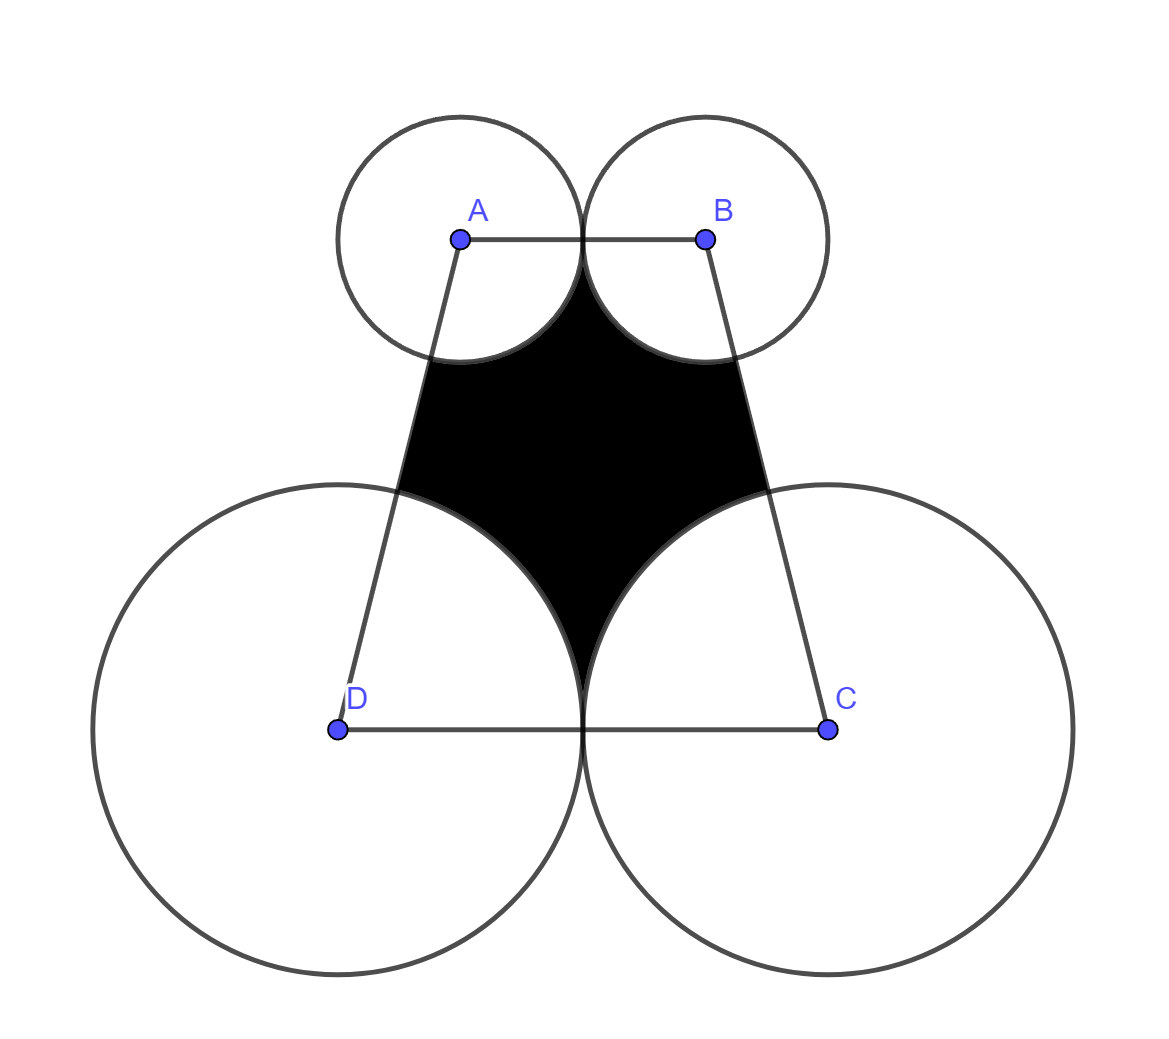
\includegraphics[scale = 0.8]{geogebra-export.png}
        \end{center}
    \item[\textbf{Bài 154.}] Cho hình ngũ giác đều nội tiếp trong đường tròn $(O)$ có bán kính $R=3,65dm$. Tính diện tích (phần màu đậm) giới hạn bởi nữa đường tròn đường kính $AB$ là cạnh của ngũ giác đều và đường tròn $(O)$.
        \begin{center}
\definecolor{ffffff}{rgb}{1,1,1}
\definecolor{uququq}{rgb}{0.25098039215686274,0.25098039215686274,0.25098039215686274}
\begin{tikzpicture}[line cap=round,line join=round,>=triangle 45,x=1cm,y=1cm, scale = 0.7]
\clip(-11.581064871867692,-4.350119651272432) rectangle (12.86578958324234,5.289251189648401);
\draw [line width=0.8pt] (0,0) circle (4cm);
\draw [line width=0.8pt] (0,4)-- (-3.804226065180614,1.2360679774997896);
\draw [line width=0.8pt] (-3.804226065180614,1.2360679774997896)-- (-2.3511410091698925,-3.2360679774997894);
\draw [line width=0.8pt] (-2.3511410091698925,-3.2360679774997894)-- (2.351141009169892,-3.23606797749979);
\draw [line width=0.8pt] (3.804226065180614,1.236067977499789)-- (2.351141009169892,-3.23606797749979);
\draw [line width=0.8pt] (0,4)-- (3.804226065180614,1.236067977499789);
\draw [shift={(-1.902113032590307,2.618033988749895)},line width=0.8pt,fill=black,fill opacity=1]  (0,0) --  plot[domain=0.6283185307179586:3.7699111843077517,variable=\t]({1*2.3511410091698925*cos(\t r)+0*2.3511410091698925*sin(\t r)},{0*2.3511410091698925*cos(\t r)+1*2.3511410091698925*sin(\t r)}) -- cycle ;
\draw [shift={(0,0)},line width=0.8pt,color=ffffff,fill=ffffff,fill opacity=1]  (0,0) --  plot[domain=1.5707963267948966:2.827433388230814,variable=\t]({1*4*cos(\t r)+0*4*sin(\t r)},{0*4*cos(\t r)+1*4*sin(\t r)}) -- cycle ;
\draw [line width=0.8pt] (0,4)-- (-3.804226065180614,1.2360679774997896);
\draw [line width=0.8pt] (0,4)-- (0,0);
\draw [line width=0.8pt] (0,0)-- (-3.804226065180614,1.2360679774997896);
\begin{scriptsize}
\draw [fill=uququq] (0,0) circle (1.5pt);
\draw[color=uququq] (0.12446647335859942,0.2543407166561644) node {$O$};
\draw [fill=black] (0,4) circle (1.5pt);
\draw[color=black] (0.12446647335859942,4.248917691646746) node {$A$};
\draw [fill=uququq] (-3.804226065180614,1.2360679774997896) circle (1.5pt);
\draw[color=uququq] (-3.6807124554039765,1.4940370192394483) node {$B$};
\draw [fill=uququq] (-2.3511410091698925,-3.2360679774997894) circle (1.5pt);
\draw[color=uququq] (-2.234400102390147,-2.9826440734224104) node {$C$};
\draw [fill=uququq] (2.351141009169892,-3.23606797749979) circle (1.5pt);
\draw[color=uququq] (2.4661150449048,-2.9826440734224104) node {$D$};
\draw [fill=uququq] (3.804226065180614,1.236067977499789) circle (1.5pt);
\draw[color=uququq] (3.9296454021211757,1.4940370192394483) node {$E$};
\end{scriptsize}
\end{tikzpicture}
        \end{center}
    \item[\textbf{Bài 155.}] Ông A gửi tiết kiệm $100$ triệu đồng với lãi suất không đổi $r=0,7\%$ một tháng. Mỗi tháng ông A phải rút ra $1$ triệu đồng để trả chi phí sinh hoạt.
        \begin{enumerate}
            \item Hỏi số tiền ông A có được sau $1$ năm là bao nhiêu.
            \item Hỏi sau bao nhiêu tháng (kể từ khi rút tiền) thì ông A không thể rút ra được số tiền lớn hơn $20$ triệu đồng.
        \end{enumerate}
    \item[\textbf{Bài 156.}] Chị Hoa vay ngân hàng $20.000.000$ đồng để kinh doanh với lãi suất $1,5\$$/tháng. Trong 2 năm đầu chị Hoa chi trả lãi hàng tháng theo lãi suất của ngân hàng, những năm còn lại chị Hoa trả $500.000$ đồng/tháng. Hỏi sau bao nhiêu tháng chị Hoa sẽ trả hết nợ.
    \item[\textbf{Bài 157.}] Một người muốn có $1.000.000$ đồng sau $15$ tháng thì mỗi tháng người đó phải gởi vào ngân hàng bao nhiêu nếu suất là $0,6\%$/tháng.
\end{enumerate}
\newpage
\end{document}